\documentclass[11pt]{beamer}


\usepackage{xcolor}

\definecolor{lightgrey}{rgb}{0.9,0.9,0.9}

\definecolor{mediumred}{rgb}{1.0,0.7,0.7}
\definecolor{lightred}{rgb}{1.0,0.9,0.9}

\definecolor{mediumgreen}{rgb}{0.7,1.0,0.7}
\definecolor{lightgreen}{rgb}{0.95,1.0,0.9}

\definecolor{darkgreen}{rgb}{0,0.6,0}


\usepackage{tipa}

\usepackage{listings}
\lstnewenvironment{latexCode}{%
  \lstset{%
    language=[latex]tex,
    texcsstyle=*\bf\color{blue},
    numbers=none,
    breaklines=true,
    keywordstyle=\color{darkgreen},
    commentstyle=\color{red},
    % otherkeywords={$, \{, \}, \[, \]},
    % frame=none,
    % tabsize=2,
    backgroundcolor=\color{lightgrey},
    % caption=LaTeX example
    basicstyle=\footnotesize\tt,
  }%
}{}


\lstnewenvironment{shell}{%
  \lstset{
    basicstyle=\tt,
    backgroundcolor=\color{lightgrey},
    emph={sage:, vbraun@laptop},
    emphstyle=\color{gray}\bfseries,
    keywordstyle=\color{blue},
    stringstyle=\color{red},
    commentstyle=\color{gray}\slshape,
  }%$
}{}

\lstnewenvironment{smallshell}{%
  \lstset{%
    basicstyle=\scriptsize\tt,
    backgroundcolor=\color{lightgrey},
    emph={vbraun@laptop},
    emphstyle=\color{gray}\bfseries,
    keywordstyle=\color{blue},
    stringstyle=\color{red},
    commentstyle=\color{gray}\slshape,
  }%$
}{}


\lstnewenvironment{tinyshell}{%
  \lstset{%
    basicstyle=\tiny\tt,
    backgroundcolor=\color{lightgrey},
    emph={vbraun@laptop},
    emphstyle=\color{gray}\bfseries,
    keywordstyle=\color{blue},
    stringstyle=\color{red},
    commentstyle=\color{gray}\slshape,
  }%$
}{}



\lstnewenvironment{bash}{%
  \lstset{%
    language=bash,
    otherkeywords={=, +, [, ], (, ), \{, \}, *},
    % bash commands from:
    %http://www.math.montana.edu/Rweb/Rhelp/00Index.html
    emph={addgroup,adduser,alias,
    ant,
    apropos,apt-get,aptitude,aspell,awk,
    basename,bash,bc,bg,break,builtin,bzip2,cal,case,cat,cd,cfdisk,chgrp,
    chkconfig,chmod,chown,chroot,cksum,clear,cmp,comm,command,continue,
    cp,cron,crontab,csplit,cut,date,dc,dd,ddrescue,declare,df,diff,diff3,
    dig,dir,dircolors,dirname,dirs,dmesg,du,echo,egrep,eject,enable,env,
    ethtool,eval,exec,exit,expand,expect,export,expr,false,fdformat,
    fdisk,fg,fgrep,file,find,fmt,fold,for,format,free,fsck,ftp,function,
    fuser,gawk,getopts,
    git,
    grep,groups,gzip,
    gunzip,
    ,hash,head,help,history,hostname,
    id,if,ifconfig,ifdown,ifup,import,install,
    java, java6, java_cur
    join,kill,killall,less,
    let,ln,local,locate,logname,logout,look,lpc,lpr,lprint,lprintd,
    lprintq,lprm,ls,lsof,make,man,mkdir,mkfifo,mkisofs,mknod,mmv,more,
    mount,mtools,mtr,mv,
    mysql,
    netstat,nice,nl,nohup,notify-send,
    noweb,noweave,
    nslookup,op,
    open,passwd,paste,pathchk,ping,pkill,popd,pr,printcap,printenv,
    printf,ps,pushd,pwd,quota,quotacheck,quotactl,ram,rcp,read,
    readarray,readonly,reboot,remsync,rename,renice,return,rev,rm,rmdir,
    rsync,scp,screen,sdiff,sed,select,seq,set,sftp,shift,shopt,shutdown,
    sleep,slocate,sort,source,split,ssh,strace,su,sudo,sum,
    svn, svn2git,
    symlink,sync,
    tail,tar,tee,test,time,times,top,touch,tr,traceroute,trap,true,
    tsort,tty,type,ulimit,umask,umount,unalias,uname,unexpand,uniq,
    units,
    unrar,
    unset,unshar,until,useradd,usermod,users,uudecode,uuencode,
    vdir,vi,vmstat,watch,wc,Wget,whereis,which,while,who,whoami,write,
    zcat},
    breaklines=true,
    keywordstyle=\color{blue},
    stringstyle=\color{red},
    emphstyle=\color{black}\bfseries,
    commentstyle=\color{gray}\slshape,
  }
}{}




\usetheme[
pagecounter=true,
pageofpages=of,  % page 7 "of" 9
bullet=circle,
titleline=true,
alternativetitlepage=true,
titlepagelogo=images/oxford_big_square,
% titlepagefooterlogo=images/oxford_small_square,
ordinarypageslogo=images/oxford_small_square,
% watermark=images/oxford_small_square,   % bottom right corner
% watermarkheight=100pt,
% watermarkheightmult=4,
]{Torino}
\usecolortheme{greenandblue}
\usefonttheme{structurebold}

\setbeamertemplate{blocks}[rounded][shadow=false]

\setbeamercolor{block body}{bg=lightgreen}
\setbeamercolor{block title}{bg=divider1}

\setbeamercolor{block body alerted}{bg=lightred,fg=black}
\setbeamercolor{block title alerted}{bg=mediumred,fg=black}


\newcommand{\cmd}[1]{\textcolor{blue}{\texttt{#1}}}


%%% Local Variables:
%%% TeX-master: "talk.tex"
%%% eval: (TeX-PDF-mode 1)
%%% End:

 


\author{Volker Braun}
\title{Git and/or the New Sage Development Workflow}
\subtitle{Making distributed version control work for you}
\institute{Oxford University}
\date{September 23, 2013}

\begin{document}


\begin{frame}[plain]
	\titlepage
\end{frame}

\section{Introduction to Git}
\begin{frame}{Outline}
	\tableofcontents
\end{frame}


\subsection{Introduction}

\begin{frame}[fragile]
  \frametitle{Linguistic Approach}
  \vspace{-5mm}
  
  \begin{block}{}
    git \textipa{/gIt/}\\
    \textit{v Appalachian \& southern US}\\
    \hspace{1cm} variant of \emph{get}\\
    \textit{n Brit slang pejorative}\\
    \hspace{1cm} foolish or worthless person
  \end{block}
  \bigskip
  \pause

  \small
\begin{verbatim}
GIT(1)                   Git Manual                   GIT(1)

NAME
       git - the stupid content tracker

SYNOPSIS
       git [--version] [--help] [-c <name>=<value>]
           [--exec-path[=<path>]] [--html-path] [--man-path]
           ...
\end{verbatim}

\end{frame}


\begin{frame}
  \frametitle{Git, the DVCS}

  \begin{itemize}
  \item 
    Developed in 2005 to manage the Linux source code
    \begin{quote}
      I'm an egotistical bastard, and I name all my projects after
      myself. First ``Linux'', now ``git'' -- Linus Torvalds
    \end{quote}
  \item Slated to overtake \emph{Subversion} as the most popular VCS
    this year.
  \item \textbf{D}istributed -- there is no central server
  \item \textbf{V}ersion \textbf{C}ontrol \textbf{S}ystem -- manage
    changes to documents
  \item Git is free and open: \url{http://git-scm.com}
  \item Official \texttt{git} implementation: command-line program
  \item Various graphical user interfaces; I like \cmd{gitg} and \cmd{git-cola}
  \item Various websites offer git hosting (Github, Bitbucket,
    Mathematical Institute \url{https://git.maths.ox.ac.uk})
  \end{itemize}

\end{frame}



\begin{frame}
  \frametitle{Demo}
  
  Introduce the following commands:
  \begin{itemize}
  \item 
    Copy repository from github:\\
    \cmd{git clone}
    \\\hfill
    \cmd{https://github.com/vbraun/talk-git-sage-workflow.git}
  \item View history:\\
    \cmd{git log}
  \item Show current branch:\\
    \cmd{git branch}
  \item Switching between branches:\\
    \cmd{git checkout master}\\\cmd{git checkout my\_branch}
  \end{itemize}
\end{frame}



%%% Local Variables:
%%% TeX-master: "talk.tex"
%%% eval: (TeX-PDF-mode 1)
%%% End:


\subsection{Basic Git Concepts}


\begin{frame}
  \frametitle{The Git Directed Acyclic Graph}

  Whenever you run \cmd{git commit}, a snapshot of the current
  state\footnote{Of the \emph{staging} directory tree, see next
    slide.} is added to the repository.
  \begin{itemize}
  \item<2-> Only forward: you can add commits, but never remove them.
  \item<3-> But: you can abandon them.
  \item<4-> Most of the time, commits have one (direct) parent commit and
    one child commit.
  \item<5-> Multiple parents: \emph{Merge} commit
  \item<6-> Multiple children: number can always increase in the future...
  \end{itemize}
\end{frame}


{
  \usebackgroundtemplate{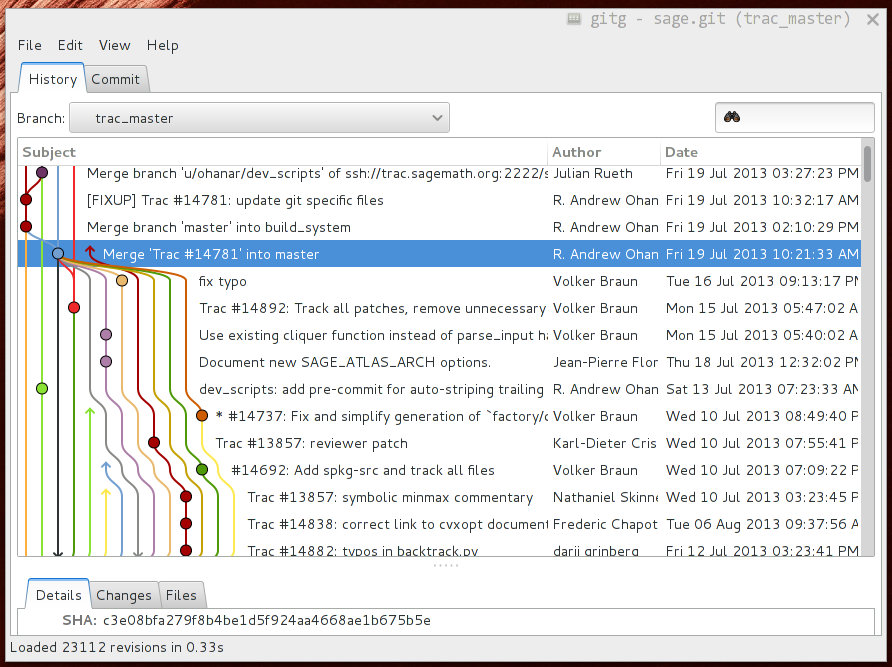
\includegraphics[width=\paperwidth]{images/gitg_screenshot}}
  \begin{frame}[plain]
    % 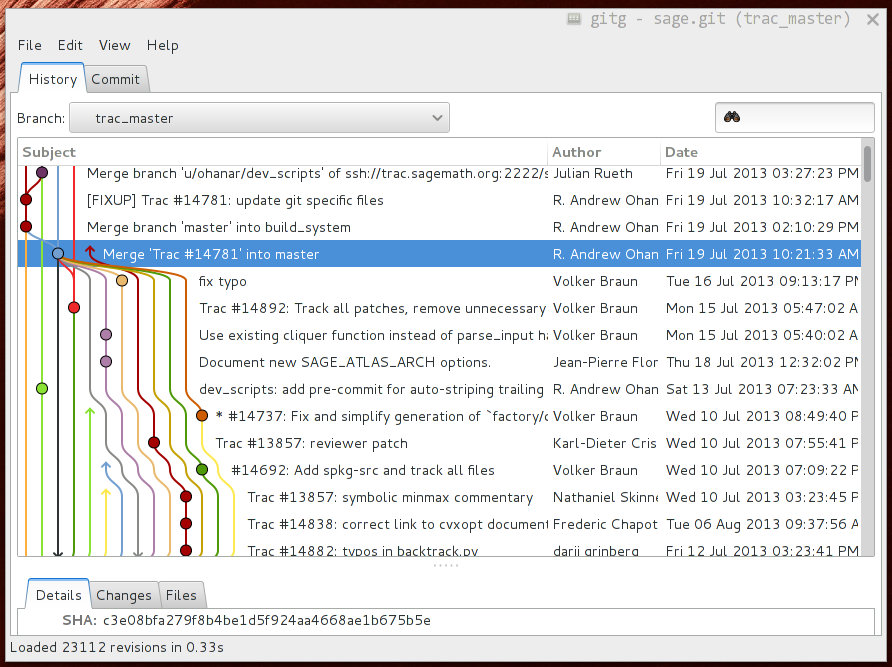
\includegraphics{images/gitg_screenshot}
  \end{frame}
}


\begin{frame}
  \frametitle{The Staging Area}

  Three places to store files:
  \begin{itemize}
  \item<2-> The git database (the \texttt{.git} directory)
  \item<3-> Staging area
  \item<4-> The working directory: all files outside of \texttt{.git} 
  \end{itemize}
  
  \onslide<5->{
    \begin{block}{Staging area}
      The staging area are the files that will be committed by
      \cmd{git commit}
      \begin{itemize}
      \item Show staging: \cmd{git status}
      \item Add to staging: \cmd{git add <filename>}
      \item Remove from staging: \cmd{git reset HEAD <filename>}
      \end{itemize}
    \end{block}
  }
\end{frame}




\begin{frame}
  \frametitle{Committing Changes}

  \begin{block}{Creating a commit}
    \begin{itemize}
    \item 
      \cmd{git commit}
    \item Specify commit message on the command line:\\
      \cmd{git commit -m "my commit message"}
    \end{itemize}
  \end{block}
  
  \onslide<2->{
    Each commit is uniquely specified by the SHA1 hash\footnote{a 40
      digit hex number} of
  }
  \begin{itemize}
  \item<2-> All changes to files
  \item<3-> All parent commits
  \item<4-> The commit message
  \end{itemize}
  \onslide<5->{
    None of these can ever be changed, including all direct and indirect
    parents.
  }
\end{frame}


\begin{frame}
  \frametitle{Branches}

  Branches organize parallel development
  \begin{itemize}
  \item<2-> A branch is just a shortcut for a particular commit
  \item<3-> If you create a new commit, the branch automatically advances
    to it
  \item<4-> The default branch is \texttt{master}, but you can use any name
  \item<5-> \texttt{HEAD} is the commit at the tip of the branch:\\
    \cmd{git show HEAD}
  \item<6-> \texttt{HEAD$\sim$} is the parent of \texttt{HEAD}
  \item<7-> \texttt{HEAD$\sim$2} is the parent of the parent of
    \texttt{HEAD}
  \item<7-> etc.
  \end{itemize}
\end{frame}


\begin{frame}
  \frametitle{Remote Repositories}
  
  \begin{itemize}
  \item<1-> Remotes repositories are bookmarks.
  \item<2-> Configure with \cmd{git remote}
  \item<3-> \textbf{D}istributed VCS: all remotes are equal.
  \item<4-> The "important" one (to you) is usually called \texttt{origin}
  \end{itemize}

  \onslide<5->{
    If there are no conflicts:
  }
  \begin{itemize}
  \item<5-> Upload your changes to the remote repository:\\
    \cmd{git push <remote>}
  \item<6-> Download changes from the remote repository and update the
    local working directory:\\
    \cmd{git pull <remote>}
  \item<7-> There is a default remote for each branch, see\\
    \cmd{git remote show <remote>}
  \end{itemize}

\end{frame}






%%% Local Variables:
%%% TeX-master: "talk"
%%% eval: (TeX-PDF-mode 1)
%%% End:


\section{Conflict Resolution}


\begin{frame}[fragile]
  \frametitle{Merge Conflicts}
  
  \begin{center}
    \Large Don't Panic!
  \end{center}

  \begin{itemize}
  \item 
    Merge conflicts happen if there are overlapping edits.
  \item 
    Resolving them is common and easy.
  \end{itemize}
  
  Example:
  \begin{latexCode}
    \begin{equation}
      \label{eq:quad}
      x = \frac{-b+-\sqrt{b^2-4ac}}{2a}
    \end{equation}
    are the two roots of the quadratic equation.
  \end{latexCode}
  
\end{frame}



\begin{frame}[fragile]
  
  On the flight to a conference I change this to
  \begin{latexCode}
    \begin{equation}
      \label{eq:quad}
      x_{1,2} = \frac{-b+-\sqrt{b^2-4ac}}{2a}
    \end{equation}
    are the two roots of the quadratic equation.
  \end{latexCode}
  \medskip
  \pause
  
  Meanwhile, Jennifer corrects
  \begin{latexCode}
    \begin{equation}
      \label{eq:quad}
      x = \frac{-b\pm\sqrt{b^2-4ac}}{2a}
    \end{equation}
    are the two roots of the quadratic equation.
  \end{latexCode}
  and pushes it to our common remote repository.
  
\end{frame}




%%% Local Variables:
%%% TeX-master: "talk"
%%% eval: (TeX-PDF-mode 1)
%%% End:




\section{Git and the Sage Workflow}
\begin{frame}{Outline}
	\tableofcontents
\end{frame}

\subsection{Setting Up}


\begin{frame}[fragile]
  \frametitle{Who Are You?}

  Your name and email address become part of the commit message 
  \begin{itemize}
  \item Global configuration stored in $\sim$\verb#/.gitconfig#. Either
    open in your favorite editor to add
    \begin{shell}
    [user]
        name = Your Name
        email = you@host.com
    \end{shell}
  \item or via the command line:
    \begin{shell}
git config --global user.name "Your Name"
git config --global user.email you@host.com
    \end{shell}    
  \end{itemize}

\end{frame}


\begin{frame}[fragile]
  \frametitle{Trac Account}
  
  To contribute to Sage, you need 
  \begin{itemize}
  \item a trac account, see instructions at \url{http://trac.sagemath.org}
  \item upload your ssh \emph{public} key to the trac server
  \item This is described in detail in
    \url{http://sagemath.github.io/git-developer-guide/trac.html#authentication},
    a temporary copy of the new developer guide.
  \end{itemize}
  
\end{frame}



\subsection{Using Git for Sage}


\begin{frame}
  \frametitle{Obtaining the Sage Sources}
  
  \begin{itemize}
  \item 
    Download the Sage git repository from github:\\
    \cmd{git clone git://github.com/sagemath/sage.git}
  \item 
    Setup the ``trac'' remote:\\
    {
      \cmd{cd sage}\\
      \cmd{git remote add trac}\\
      \hfill
      \cmd{ssh://git@trac.sagemath.org:2222/sage.git -t master}
    }
  \item Note: the \cmd{-t master} means to only fetch the master
    branch by default 
    \begin{itemize}
    \item Pro: Avoids downloading all branches on trac; Faster and
      less clutter
    \item Con: You have to tell git which branches to download
    \end{itemize}
  \end{itemize}
\end{frame}




\begin{frame}
  \frametitle{Downloading a Branch from Trac}

   \begin{alertblock}{Temporary change}
     You should use the \cmd{public/sage-git/master} branch for
     now. When the git transition is finished, it well be just
     \cmd{master}.
   \end{alertblock}
   
   So, first get this branch:
   \begin{itemize}
   \item 
     Tell git which branch to download:\\
     \cmd{git fetch trac public/sage-git/master}
   \item 
     Create a new local branch from what you just downloaded:\\
     \cmd{git checkout -b trac\_master FETCH\_HEAD}
   \end{itemize}

   Then build Sage as usual (run \cmd{make})
\end{frame}


\subsection{Integration with Sage Trac}

\begin{frame}
  \frametitle{Uploading Changes}

  \begin{itemize}
  \item Now edit files and commit changes. Just like with any other git
    repository.
  \item If you have a (new or existing) ticket, fill in the
    ``Branch:'' field with the name that you will be using to upload.
  \item The remote branch name must be \cmd{u/user/description}, where
    \begin{itemize}
    \item \cmd{user} is your trac username
    \item \cmd{description} is a free-form short description (and can
      include further slashes)
    \end{itemize}
  \item 
    When you are ready to share, upload to trac:\\
    \cmd{git push --set-upstream trac}\\
    \hspace{2cm}\cmd{my\_branch:u/user/description}
  \item 
    Slightly different push command for subsequent uploads:\\
    \cmd{git push trac HEAD:u/user/description}
  \end{itemize}
\end{frame}



\begin{frame}
  \frametitle{Using Trac}

  \begin{itemize}
  \item When you push to a trac ticket, the ``Commit:'' field on the
    trac ticket is automatically filled out.
  \item The ``Branch:'' field is color coded:
    \begin{itemize}
    \item \textcolor{green}{Green} means that it applied cleanly to the current master.
    \item \textcolor{red}{Red} means that there is a conflict.
    \end{itemize}
  \item If you click on the ``(Commits)'' link under/next to the
    branch, you can see the list of commits.
  \item Download any branch for the first time as on the ``Downloading
    a Branch from Trac'' slide.
  \item To get changes, use \cmd{git pull trac u/user/description}
  \end{itemize}
\end{frame}


{
  \usebackgroundtemplate{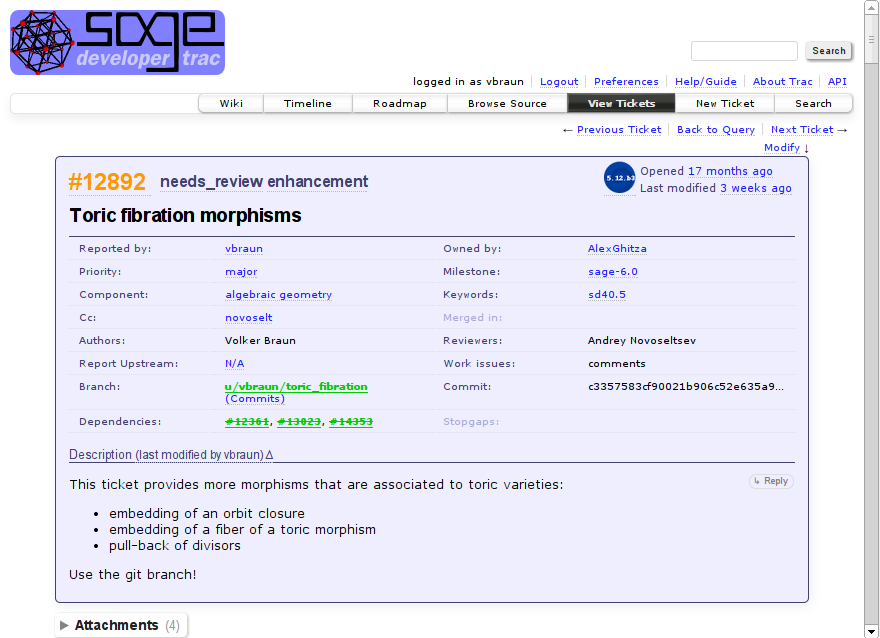
\includegraphics[width=\paperwidth]{images/trac_screenshot}}
  \begin{frame}[plain]
  \end{frame}
}




\begin{frame}[fragile]
  \frametitle{Merging vs.\ Rebasing}

  While you are working on \cmd{my\_branch}, Sage development
  continues.
\begin{verbatim}
             X---Y---Z my_branch
            /
       A---B---C---D master
\end{verbatim}
  Two ways to update:
  \begin{itemize}
  \item Merge: \cmd{git merge master}
\begin{verbatim}
             X---Y---Z---W my_branch
            /           /
       A---B---C-------D master
\end{verbatim}
  \item Rebase: \cmd{git rebase master}
\begin{verbatim}
                     X'--Y'--Z' my_branch
                    /
       A---B---C---D master
\end{verbatim}
  \end{itemize}
  
\end{frame}





\begin{frame}[fragile]
  \frametitle{Rebasing}
  
    \begin{itemize}
    \item Rebase: \cmd{git rebase master}
\begin{verbatim}
                     X'--Y'--Z' my_branch
                    /
       A---B---C---D master
\end{verbatim}
    \item Pro: Clean history.
    \item Con: Since the SHA1 hash includes the hash of the parent,
      all commits change.
    \item Only ever use rebase if nobody else has used one of your
      \texttt{X}, \texttt{Y}, \texttt{Z} commits to base their
      development on.
    \item Only rebase commits that you have not yet pushed to trac.
  \end{itemize}
  
\end{frame}





\begin{frame}[fragile]
  \frametitle{Merging}
  
    \begin{itemize}
  \item Merge: \cmd{git merge master}
\begin{verbatim}
             X---Y---Z---W my_branch
            /           /
       A---B---C-------D master
\end{verbatim}
      \item Pro: None of the existing commits changes
      \item Con: Introduces a new commit \texttt{W} that will be in the
        \cmd{git log} history forever.
      \item When you push to trac, the extra commit propagates to your
        collaborators. 
      \item When in doubt, use merge instead of rebase.
  \end{itemize}
  
\end{frame}







%%% Local Variables:
%%% TeX-master: "talk.tex"
%%% eval: (TeX-PDF-mode 1)
%%% End:





\section{The Sage Dev Scripts}
\begin{frame}{Outline}
	\tableofcontents
\end{frame}




\section{Summary}

\begin{frame}
  
\includegraphics[width=0.6\linewidth]{images/git_logo}
  \hfill
  
\includegraphics[width=0.3\linewidth]{images/sagemath_icon}
  \hfill
  \vspace{1cm}

  \begin{center}
    \Huge
    The End. Questions?
  \end{center}
\end{frame}

\begin{frame}[plain]
  \frametitle{Git Operations}
  \centering
  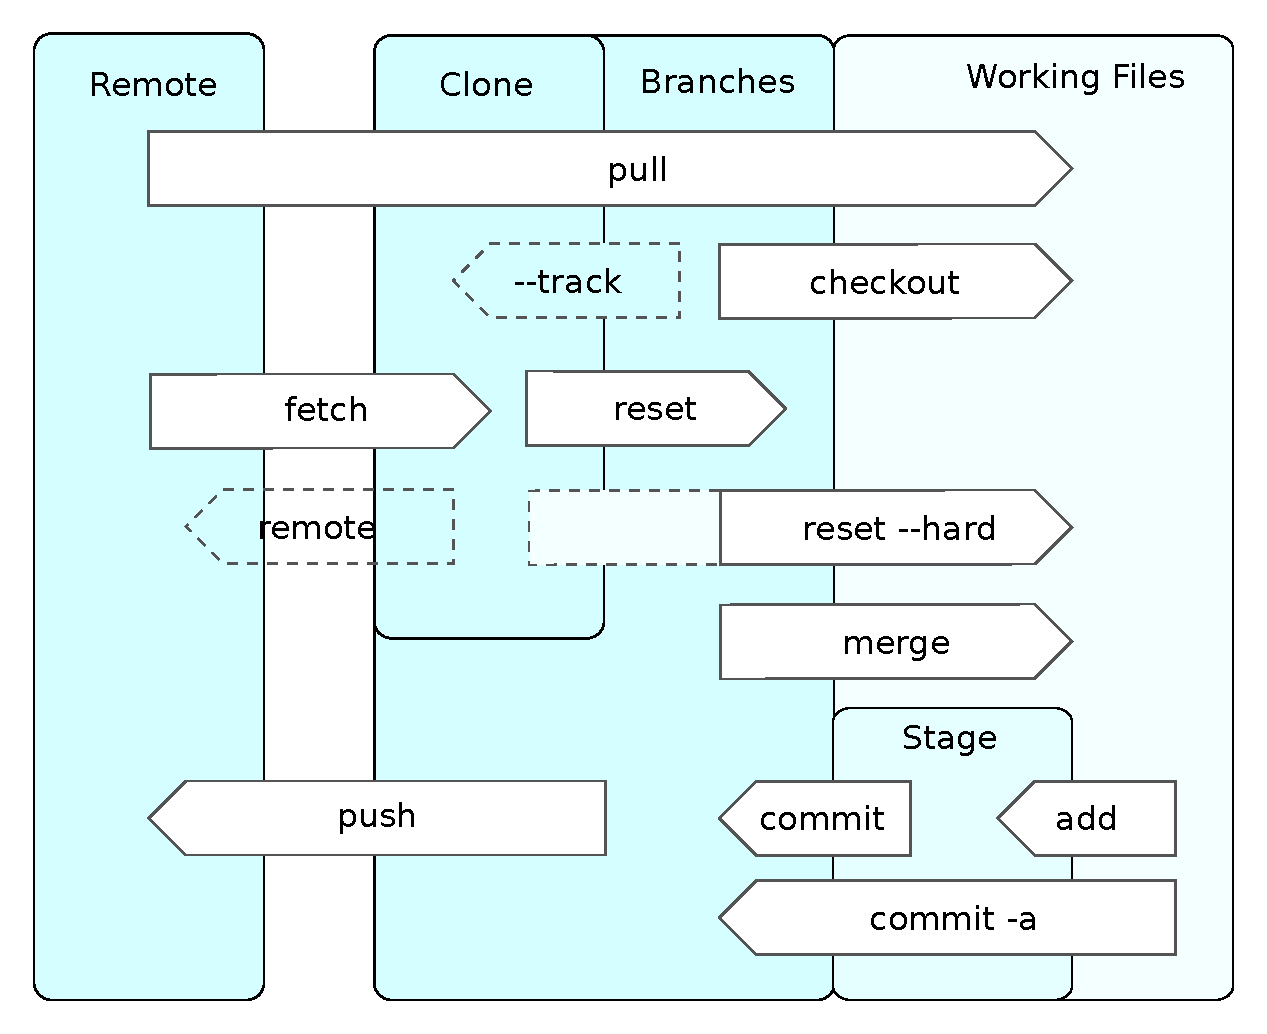
\includegraphics[width=0.85\linewidth]{images/git_operations}
\end{frame}




\end{document}


%%% Local Variables:
%%% eval: (TeX-PDF-mode 1)
%%% End:
